
\documentclass[handout]{beamer}

%\usepackage[table]{xcolor}
\mode<presentation> {
  \usetheme{Boadilla}

%  \usetheme{Pittsburgh}
%\usefonttheme[2]{sans}
\renewcommand{\familydefault}{cmss}
%\usepackage{lmodern}
%\usepackage[T1]{fontenc}
%\usepackage{palatino}
%\usepackage{cmbright}
  %\setbeamercovered{transparent}
\useinnertheme{rectangles}
}

\setbeamercolor{normal text}{fg=black}
\setbeamercolor{structure}{fg= blue}
\definecolor{trial}{cmyk}{1,0,0, 0}
\definecolor{trial2}{cmyk}{0.00,0,1, 0}
\definecolor{darkgreen}{rgb}{0,.4, 0.1}
\usepackage{array}
\beamertemplatesolidbackgroundcolor{white}  \setbeamercolor{alerted
text}{fg=red}
\usepackage{tcolorbox}
\setbeamertemplate{caption}[numbered]\newcounter{mylastframe}


\usepackage{tikz}
\usetikzlibrary{arrows}
\usepackage{colortbl}

\renewcommand{\familydefault}{cmss}
%\usepackage[all]{xy}

\usepackage{tikz}
\usepackage{lipsum}

 \newenvironment{changemargin}[3]{%
 \begin{list}{}{%
 \setlength{\topsep}{0pt}%
 \setlength{\leftmargin}{#1}%
 \setlength{\rightmargin}{#2}%
 \setlength{\topmargin}{#3}%
 \setlength{\listparindent}{\parindent}%
 \setlength{\itemindent}{\parindent}%
 \setlength{\parsep}{\parskip}%
 }%
\item[]}{\end{list}}
\usetikzlibrary{arrows}

\usecolortheme{lily}

\newtheorem{com}{Comment}
\newtheorem{lem} {Lemma}
\newtheorem{prop}{Proposition}
\newtheorem{condition}{Condition}
\newtheorem{thm}{Theorem}
\newtheorem{defn}{Definition}
\newtheorem{cor}{Corollary}
\newtheorem{obs}{Observation}
 \numberwithin{equation}{section}
 

\setbeamertemplate{navigation symbols}{}


\title[PLSC 43401]{Mathematical Foundations of Political Methodology}

\author{Robert Gulotty}
\institute[Chicago]{University of Chicago}
\vspace{0.3in}




\begin{document}

\begin{frame}
\maketitle
\end{frame}

\begin{frame}
\frametitle{Lecture 11 Conditional probability}

\begin{itemize}
\item Conditional Probability
\item Bayes Rule
\item Independence
\end{itemize}
\end{frame}

\begin{frame}{Why study conditional probability?}

Most of the relationships we are interested in as policy makers/analysts, are conditional ones. Knowing that an event has occurred might lead us to reassess the probability of another event.\pause

\begin{itemize}
\item What is the probability of Iran obtaining nuclear weapons given that it has a uranium enrichment program?\pause
\item What is the probability that we will be able to affect climate change if we adopt the climate change treaty?\pause
\item What is the probability of holding liberal political views given certain demographic characteristics?
\end{itemize}
\end{frame}

\begin{frame}
\frametitle{Definition of Conditional probability}
The \emph{conditional probability} of an event A given an event B is given by:
$$P(A|B)=\frac{P(A\cap B)}{P(B)}$$
for all $P(B)\neq 0$\\
\pause We can rearrange this to form the``Multiplication Rule'':
$$P(A\cap B)=P(A|B)\times P(B)$$

\end{frame}





\begin{frame}
\frametitle{Examples of Conditional Probability} 

Example 1: \pause  
\begin{itemize}
\item[-] $F = \{\text{Myanmar sells oil to China} \} $\\  \pause 
\item[-] $E = \{\text{Myanmar discovers oil} \} $ \\   \pause 
\item[-] If $F$ occurs then $E$ must occur, $P(E|F) = 1$ \\  \pause 
\end{itemize}


Example 2: Security Council voting on Syria strike \pause 
\begin{itemize}
\item[-] $V = \{ \text{Russia and China veto strike}\} $\pause
\item[-] $A = \{ \text{Strike approved by UN}\}$  \pause 
\item[-] $P(A|V)  = \frac{P(A \cap V)}{P(V) } = \frac{P(\emptyset)}{P(V)}$ = 0
\end{itemize}


\end{frame}







\begin{frame}
\frametitle{Axioms of Conditional probability}
$P(A|B)$ is a probability, so it follows the axioms.
\begin{enumerate}
\item $P(A|B)\geq 0, \ \ \forall A$
\item $P(\Omega|B)=1$.
\item For all mutually exclusive events, $A_1,\ A_2,\ ... A_n$
$$P(A_1\cup A_2 \cup...\cup A_n|B)= P(A_1|B)+P(A_2|B)+...+ P(A_n|B)$$
\end{enumerate}
\end{frame}

\begin{frame}
\frametitle{Conditional Probability Example}
Basic claim: Foreign military threats (given certain other conditions) produce revolutions.
\begin{itemize}
\item Skocpol (1979)
\item Let E denote the event of a revolution and
\item Let F the presence of a foreign threat 
\end{itemize}\pause
The way to read Skocpol's hypothesis in probability language is:\\
$P(E|F)\geq P(E|F^c)$

\end{frame}


\begin{frame}
\frametitle{Conditional Probability Example}
How might we know whether $P(E|F)>P(E|F^c)?$\pause
\begin{itemize}
\item $P(E|F)=\frac{P(E\cap F)}{P(F)}$
\item $P(E|F^c)=\frac{P(E\cap F^c)}{P(F^c)}$\pause
\item So we need to know both the rate of Revolutions with foreign threats, the rate of Revolutions without foreign threats, and the probability of a foreign threat.
\end{itemize}

\end{frame}

\begin{frame}
\frametitle{Revolutions}
Skocpol's data:\\
\vspace{1 cm}

\begin{tabular}{r|cc}
&Revolution&No Revolution\\
\hline
Foreign Threat& France, Russia, China\\
No Threat&& England, Prussia, Japan\\
\end{tabular}
\end{frame}



\begin{frame}
\frametitle{$P(A|B)$ and $P(B|A)$ are different}

$$P(A|B) = \frac{P(A\cap B)}{P(B)}$$\pause
$$P(B|A)  =  \frac{P(A \cap B) } {P(A)}$$\pause
$$P(A|B)  =  \frac{P(B|A)P(A)} {P(B)} $$
\end{frame}


\begin{frame}
\frametitle{Example 1}
$$P(\text{Tall}|\text{Professional Basketball Player})=.9$$
$$P(\text{Professional Basketball Player}|\text{Tall})=.00002$$


\end{frame}


\begin{frame}
\frametitle{Example 2}

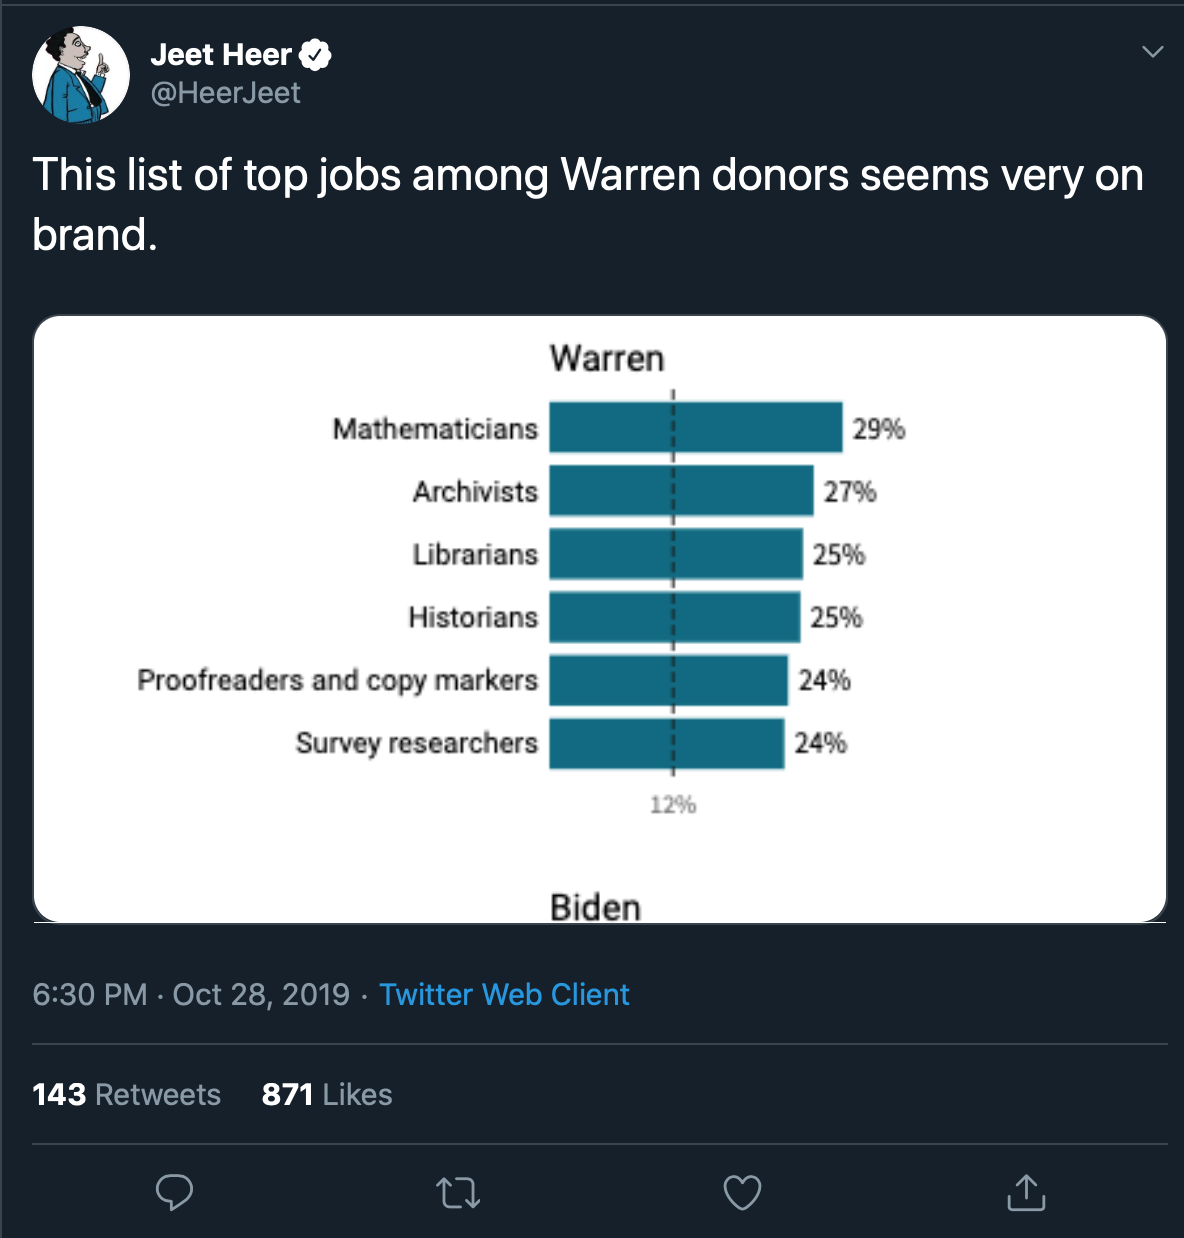
\includegraphics[width=3 in]{JeetTweet.png}


\end{frame}



\begin{frame}
\begin{prop} 
Multiplication Rule: 
Suppose $E_{1}, E_{2}, \hdots, E_{N}$ is a sequence of events.  
\begin{eqnarray}
P(E_{1}\cap E_{2}\cap \cdots \cap E_{N} ) & =& \nonumber \\
P(E_{1})P(E_{2}|E_{1}) P(E_{3}|E_2, E_{1} ) \times \cdots \times P(E_{N} | E_{N-1}, E_{N-2} , \hdots, E_{1} )  && \nonumber
\end{eqnarray}
\end{prop} 

\pause 
\begin{proof} 
\begin{small}
\begin{eqnarray}
P(E_{1}) P(E_{2}| E_{1} ) & = & P(E_{1}) \frac{P(E_{2} \cap E_{1} )}{P(E_{1})} \quad \textbf{Def of CP} \nonumber \\
& = & P(E_{1} \cap E_{2} ) \nonumber \\ \pause 
P(E_{1} \cap E_{2} ) P(E_{3}| E_{1}, E_{2} ) &= & P(E_{1} \cap E_{2} ) \frac{P(E_{3} \cap E_{2} \cap E_{1} )  }{P(E_{2} \cap E_{1} ) } \nonumber \\
& = & P(E_{3} \cap E_{2} \cap E_{1} )  \nonumber  \pause 
\end{eqnarray}
Repeating for all probabilities proves the proposition

\end{small}

\end{proof}


\end{frame}


\begin{frame}
\frametitle{Law of Total Probability}

For a set of mutually exclusive events, $E_1,\  E_2,\ E_3 .... E_n$, which together form the sample space $\Omega$, the probability of any event A is:

$$P(A)= P(A|E_1)P(E_1)+P(A|E_2)P(E_2)+...+P(A|E_n)P(E_n)$$
\pause
\begin{proof} 
\begin{small}
\begin{eqnarray}
P(A)& = &P(A\cap \Omega)  \nonumber  \\\pause
P(A)& = &P(A\cap (E_1\cup E_2 \cup ... \cup E_n))  \nonumber \\\pause
P(A)& = &P((A\cap E_1)\cup (A\cap E_2) \cup ... \cup(A\cap E_n)) \nonumber\\ \pause
P(A)& = & P(A\cap E_1)+ P(A\cap E_2) + ...P(A\cap E_n) \nonumber \\\pause
P(A)& = & P(A|E_1)P(E_1)+P(A|E_2)P(E_2)+...+P(A|E_n)P(E_n) \nonumber 
\end{eqnarray}
\end{small}

\end{proof}


\end{frame}


\begin{frame}
\frametitle{Example: Law of Total Probability}
 Say you decide to implement a Democracy Promotion Program (DPP) in some villages in Myanmar in the hopes of increasing voter turnout at the next election. What is P(vote) after DPP?\pause
 \begin{itemize}
 \item Let $P(vote|DPP)=0.6$\pause
 \item Let $P(vote|\sim DPP)=0.3$\pause
 \item Let $P(DPP) = P(\sim DPP) = 0.5$ (Decided based on coin-flipping)\pause
 \item $P(vote)= .6*.5+.3*.5= .45$
 \end{itemize}
\end{frame}


\begin{frame}
\frametitle{Example: Law of Total Probability} 

Infer $P(\text{vote})$ after mobilization campaign \pause 
\begin{itemize}
\item[-] $P(\text{vote}|\text{mobilized} ) = 0.75$ \pause 
\item[-] $P(\text{vote}| \text{not mobilized} ) = 0.25 $ \pause 
\item[-] $P(\text{mobilized}) = 0.6 ; P(\text{not mobilized} ) = 0.4 $ \pause 
\item[-] What is $P(\text{vote})$? \pause 
\end{itemize}

Sample space (one person) = \\$\{$ (mobilized, vote), (mobilized, not vote), (not mobilized, vote) , (not mobilized, not vote) $\}$\\
\alert{Mobilization} partitions the space (mutually exclusive and exhaustive)  \pause \\
We can use the law of total probability \pause 
\begin{eqnarray}
P(\text{vote} ) & = & P(\text{mob.} ) \times P(\text{vote}| \text{mob.} ) + P(\text{not mob}) \times P(\text{vote} | \text{not mob} ) \nonumber \\
 & = & 0.6 \times 0.75 + 0.4 \times 0.25 \nonumber \\
  & = & 0.55 \nonumber 
  \end{eqnarray}

\end{frame}


\begin{frame}
\frametitle{Example Law of Total Probability}

\alert{Mixture Models}: flexible modeling strategy.  \\ \pause 

Two coins:\\ \pause 
\begin{itemize}
\item[-] Fair: $P(H) = 1/2$  \pause
\item[-] Biased $P(H) = 3/4$ \pause 
\end{itemize}

Draw a coin from urn ($P(\text{fair}) = 1/2)$ and then flip.  \\
$P(H)?$ \pause 

$\Omega = \{(\text{fair}, H), (\text{fair}, T), (\text{bias}, H), (\text{bias}, T) \}$ \pause 

\begin{eqnarray}
P(H) & = & P(\text{fair}) \times P(H| \text{fair} )  + P(\text{bias} ) \times P(H | \text{bias} ) \nonumber\\ \pause 
& = & \frac{1}{2} \times \frac{1}{2} + \frac{1}{2} \times \frac{3}{4} \nonumber \\
& = & \frac{5}{8}\nonumber \pause 
\end{eqnarray}

\alert{Mixture} of two coins


\end{frame}



\begin{frame}
\frametitle{Bayes' Rule} 

\begin{itemize}
\item[-] $P(B|A)$ may be easy to obtain
\item[-] $P(A|B)$ may be harder to determine
\item[-] Bayes' rule provides a method to move from $P(B|A)$ to $P(A|B)$.  
\end{itemize}



\end{frame}

\begin{frame}
\frametitle{Conditional Probability and Bayes' Rule}
 $$P(A|B)=\frac{P(A\cap B)}{P(B)}$$
 $$P(A\cap B)=P(B\cap A)=P(B|A)P(A)$$\pause
 
 \begin{thm}{Bayes' Rule}
  $$P(A|B)=\frac{P(B|A)P(A)}{P(B)}$$
\end{thm}
\end{frame}


\begin{frame}
\frametitle{General Statement of Bayes' Rule}
Let the events $A_1...A_k$ form a partition of the space S such that $P(A_j)>0$ for $j=1...k$.
And let B be an event such that $P(B)>0$.  Then for $i=1...k$
 
 \begin{thm}{Bayes' Rule}
  $$P(A_i|B)=\frac{P(A_i)P(B|A_i)}{\sum_{j=1}^{k}P(A_j)P(B|A_j)}$$
\end{thm}
\end{frame}




\begin{frame}
\frametitle{Bayes' Rule Example} 
Suppose that the US has captured lots of foreign Islamic militants in Afghanistan:
\begin{itemize}
\item 20\% from Saudi Arabia (A)
\item 30\% from Yemen (Y)
\item 45\% from Pakistan (K)
\item 5\% from the USA (U)
\end{itemize}

\end{frame}

\begin{frame}
\frametitle{How likely is a foreign fighter to be a convert?} 
Further suppose that we know something about the probability that the foreign fighter is a `convert' to Islam \textbf{C}:
\begin{itemize}
\item $P(C|saudi Arabia)= 0.03$
\item $P(C|Yemen)= 0.05$
\item $P(C|paK)= 0.07$
\item $P(C|Usa)= 0.8 $
\end{itemize}
\end{frame}


\begin{frame}
\frametitle{How likely is a convert to be from the USA?} 

$$P(USA|C)=\frac{P(U)*P(C|U)}{P(C)}$$
$$=\frac{P(U)*P(C|U)}{P(U)*P(C|U)+P(A)*P(C|A)+P(Y)*P(C|Y)+P(K)*P(C|K)}  $$\pause
$$=\frac{.05*.8}{.05*.8+.2*.03+.3*.05+.45*.07}=.43$$

Even though 80 percent of American fighters are converts, relative to 7 percent of Pakistani or Yemeni or Saudi fighters, it is still more likely that the fighter is not from the US than from the USA.  \pause This is because it is unlikely for there to be a fighter from the US in the first place.
\end{frame}



\begin{frame}
\frametitle{Monty Hall Problem}

Suppose we have three doors.  $A, B, C$.  \pause \\
Suppose you're on a game show, and you're given the choice of three doors: Behind one door is a car; behind the others, goats. \\ \pause 
\begin{itemize}
\item[-] A contestant guesses a door. \pause 
\item[-] The host opens a different door, revealing one of two goats. The contestant has option to switch \pause 
\item[-] Should the contestant switch? \pause 
\end{itemize}

Contestant guesses $A$\\ \pause 
$P(A) = 1/3 \leadsto$ chance of winning without switch\\ \pause 
If $C$ is revealed to not have a car:\\

\end{frame}


\begin{frame}
\frametitle{Monty Hall Problem}

\pause 
\begin{eqnarray}
P(B| C \text{ revealed} ) & = & \frac{P(B)P(C \text{ revealed} | B)}{P(B)P(C \text{ revealed} | B) + P(A) P(C \text{ revealed} | A) } \nonumber \\ \pause 
& = & \frac{1/3 \times 1}{1/3 + 1/3 \times 1/2 } = \frac{1/3}{1/2} = \frac{2}{3}\nonumber \\ \pause 
P(A| C \text{ revealed} ) & = & \frac{P(A) P(C \text{ revealed} | A)}{ P(B)P(C \text{ revealed} | B) + P(A) P(C \text{ revealed} | A) }\nonumber \\ \pause 
& = & \frac{1/3 \times 1/2}{1/3 + 1/3 \times 1/2} = \frac{1}{3} \nonumber \pause 
\end{eqnarray}

\alert{You can double the chances of winning with switch}


\end{frame}



\begin{frame}{Joint Probability and Independence}

\begin{itemize}
\item In statistics, we will often seek to infer facts about the world from the outcomes of repeated experiments.\pause
\item To discover the systematic component of the experiment, we need to make assumptions about what affects what.\pause
\item The most important and stringent of these is the notion of independence.
\end{itemize}
\end{frame}


\begin{frame}{Independence}

\begin{defn}
Suppose we have two events $E_{1}, E_{2}$.  We say these events are \alert{independent} if:
\begin{eqnarray}
P(E_{1}\cap E_{2}) & = & P(E_{1}) P( E_{2}) \nonumber 
\end{eqnarray}
\end{defn}

\end{frame}



\begin{frame}

\begin{defn}
Suppose we have a sequence of events $E_{1}, E_{2}, \hdots, E_{n}$.  We say the sequence of events is \alert{mutually independent} if for each subset of the sequence,  $E_{i_{1}}, E_{i_{2}}, \hdots, E_{i_{j}}$ 
\begin{eqnarray}
P(E_{i_{1}}\cap E_{i_{2}}\cap \hdots \cap E_{i_{j}}) & = & \prod_{m = 1}^{j} P(E_{i_{m}}) \nonumber 
\end{eqnarray}
\end{defn}

\alert{For a sequence to be independent, every subset must be independent }


\end{frame}


\begin{frame}
\frametitle{Independence and Information} 

Does one event provide \alert{information} about another event? \pause 

\begin{defn} 
If learning about B does not change the probability that A occurs, A is independent of B.
 $$P(A|B)=P(A)$$\pause
 $$P(A|B)=\frac{P(A\cap B)}{P(B)}=P(A)$$
\end{defn}
\pause

Independence is symmetric: if $F$ is independent of $E$, then
  $E$ is independent of $F$

\end{frame}


\begin{frame}{Examples of Independence}

\begin{itemize}
\item Whether a red shows on the roulette wheel is independent of whether a green showed 10 times previously.\pause
\item The stock portfolio's performance relative to the market average today is independent of the performance yesterday.\pause
\item The extent of rainfall in Mexico in 1664 is independent of Spanish investments in local elites in 1620. 
\end{itemize}
\end{frame}


\begin{frame}
\frametitle{Independence}
What if A is \emph{Mutually Exclusive} of B?\pause
 $$A\cap B=\emptyset$$\pause
 
  $$P(A|B)=\frac{P(\emptyset)}{P(B)}=0\neq P(A)$$
 \pause
 If two events occur with positive probability, then they cannot be mutually exclusive and independent.
 \end{frame}




\begin{frame}
\frametitle{Example Independence Relationship}

Flip a fair coin twice.  
\begin{itemize}
\item[] $E = \text{first flip heads} $
\item[] $F = \text{second flip heads} $
\end{itemize}\pause
\begin{eqnarray}
P(E \cap F ) & = & P( \{ (H, H) , (H, T) \} \cap \{ (H, H), (T, H) \} ) \nonumber \pause \\
 & =& P( \{(H, H)\} ) \nonumber \\ 
 & = & \frac{1}{4} \nonumber \\
P(E ) & = & \frac{1} {2} \nonumber \pause \\
P(F) & = & \frac{1}{2} \nonumber \pause \\
P(E)P(F)  & =& \frac{1}{2}\frac{1}{2} = \frac{1}{4}  =P(E \cap F )  \nonumber 
 \end{eqnarray} 
 
 

\end{frame}

\begin{frame}
\frametitle{Independence: No Information} 

Suppose $E$ and $F$ are independent.  Then, 
\begin{eqnarray}
P(E|F ) & = & \frac{P(E \cap F) }{P(F) } \nonumber \\
& = & \frac{P(E)P(F)}{P(F)}\nonumber \\
& = & P(E) \nonumber 
\end{eqnarray}


Conditioning on the event $F$ does not modify the probability of $E$.  \\
\alert{No information about $E$ in F}  \\

\end{frame}



\begin{frame}
\frametitle{Independence and Compliments}

\begin{prop}
Suppose $A$ and $B$ are independent events. Then the events $A$ and $B^{c}$ are also independent.  
\end{prop}

\pause 

\begin{proof}
\begin{eqnarray}
P(A \cap B^{c} ) & = & P(A) - P(A \cap B)  \quad \textbf{LTP}\nonumber  \pause \\
& = & P(A)  - P(A) P(B)  \quad \textbf{Ind. of A and B} \nonumber  \pause \\
& = & P(A) ( 1- P(B) )  \pause \nonumber \\
& = & P(A) P(B^{c})   \nonumber 
\end{eqnarray}
\end{proof}



\end{frame}


\begin{frame}
\frametitle{Example: Independence and Causal Inference} 

Selection and Observational Studies
\begin{itemize}
\item[-] We often want to infer the effect of some treatment 
\begin{itemize}
\item[-] Incumbency on vote return 
\item[-] Democracy on war
\end{itemize}
\item[-] Observational studies: observe what we see to make inference 
\item[-] Problem: units select into treatment 
\begin{itemize}
\item[-] Simple example: enroll in job training if I think it will help 
\item[-] P(job$|$training in study) $\neq$ P(job$|$forced training) 
\end{itemize}
\item[-] \alert{Background characteristic}: difference between
  treatment and control groups
\item[-] \alert{Experiments}: make background characteristics and treatment status
  independent 
\end{itemize}


\end{frame}

\begin{frame}{Example of Independence and Causal inference.}
Example: democracy promotion programs in countries where we think they are likely to succeed\pause
Suppose a researcher got to choose where to put a democracy promotion program, and finds the following:
\begin{table}
\begin{tabular}{lll}
		&Democracy& No Democracy\\
DPP &10 & 50\\
no DPP & 2& 13\\

\end{tabular}
\end{table}
\pause
$$P(Democracy|\ DPP)= \frac{(10/75)}{(60/75)} =1/6= .17$$
$$P(Democracy| no\ DPP)=  \frac{(2 /75)}{(15/75)} = 2/15=.13$$

 \end{frame}




\begin{frame}{Example of Independence and Causal inference.}
Now if we knew that the researcher conditioned on a particular observable outcome, we could control for that variable:\pause

\begin{table}
\begin{tabular}{llll}
		&&Democracy& No Democracy\\
 Prior Good Gov & DPP &2 & 18\\
		 &no DPP & 1& 9\\
		 \hline
Prior Bad Gov  & DPP &8 & 32\\
		&no DPP & 1& 4\\



\end{tabular}
\end{table}
\pause
$$P(Democracy| DPP\& GG)= \frac{(2/75)}{( 20/75)} = .1$$
$$P(Democracy| no DPP\& GG)=  \frac{(1/75)}{(10/75)} = .1$$
\pause
$$P(Democracy| DPP\& BG)= \frac{(8/75)}{( 40/75)} = .2$$
$$P(Democracy| no DPP\& BG)=  \frac{(1/75)}{(5/75)} = .2$$
 \end{frame}




\begin{frame}
\frametitle{Conditional  Independence}

\begin{defn}
Let $E_{1}$ and $E_{2}$ be two events.  We will say that the events are conditionally independent given $E_{3}$ if 
\begin{eqnarray}
P(E_{1} \cap E_{2} | \alert{E_{3}}) & = & P(E_{1} | E_{3} ) P(E_{2} | E_{3} ) \nonumber 
\end{eqnarray}


\end{defn}



\end{frame}





\begin{frame}

\begin{prop}
Suppose $E_{1}$ and $E_{2}$ and $E_{3}$ are events such that $P(E_{1} \cap E_{2})>0$ and $P(E_{2} \cap E_{3}) >0$.  Then $E_{1}$ and $E_{2}$ are conditionally independent given $E_{3} $ \textbf{if and only if} $P(E_{1} | E_{2} \cap E_{3})  = P(E_{1} | E_{3}) $.  
\end{prop} \pause

\begin{proof}
Suppose $E_{1}$ and $E_{2}$ are conditionally independent given $E_{3}$.  Then 
\begin{eqnarray}
P(E_{1} \cap E_{2} |  E_{3}) & = & \frac{P(E_{1} \cap E_{2} \cap E_{3}  ) }{P(E_{3} )}  \quad \textbf{Def of Conditional Pr.}\nonumber \\
& = & \frac{P(E_{3})P(E_{2} | E_{3} )P(E_{1} | E_{2} \cap E_{3} ) }{ P(E_{3} )}  \quad \textbf{Mult. Rule} \nonumber \\\pause
P(E_{1}|E_{3}) P(E_{2} | E_{3} ) & = & P(E_{2} | E_{3} )P(E_{1} | E_{2} \cap E_{3} ) \nonumber \\
P(E_{1}|E_{3}) & = & P(E_{1} | E_{2} \cap E_{3} ) \nonumber 
\end{eqnarray}

\end{proof}





\end{frame}

\begin{frame}

\begin{proof}
Suppose $P(E_{1} | E_{2} \cap E_{3})  = P(E_{1} | E_{3}) $
\pause
\begin{eqnarray}
P(E_{1} \cap E_{2}| E_{3 } ) & = & P(E_{2} | E_{3} ) P(E_{1} | E_{2}\cap E_{3} ) \quad \textbf{Multiplication Rule}\nonumber \pause\\
 & = & P(E_{2} | E_{3} ) P(E_{1} | E_{3} ) \nonumber 
\end{eqnarray}

\end{proof}

\end{frame}




\begin{frame}
Going back to our democracy promotion example:
\begin{table}
\begin{tabular}{llll}
		&&Democracy& No Democracy\\
 Prior Good Gov & DPP &2 & 18\\
		 &no DPP & 1& 9\\
		 \hline
Prior Bad Gov  & DPP &8 & 32\\
		&no DPP & 1& 4\\
\end{tabular}
\end{table}\pause

$$P(E_{1} | E_{2} \cap E_{3})  = P(E_{1} | E_{3}) $$ 
$$P(Democracy| DPP\& GG) = (2/75)/(20/75)=.1$$
$$P(Democracy| GG) = (3/75)/(30/75)=.1$$

\end{frame}






\end{document}


